\documentclass[handout]{ximera}
\input{../preamble.tex}
\author{Mary E. Pilgrim, and implemented in Ximera by Liam Coulter}


\title{Spring 2017 Exam 2}

\begin{document}
\begin{abstract}
  Here you can work on a practice exam 3. This exam was administered in Spring 2017.
\end{abstract}
\maketitle

\begin{center}
\Large{Math 160 Calculus for Physical Scientists I \\ Exam 2 - Version 1 \\ April 13, 2017, 5:00-6:50 pm}
\end{center}


%%MC%%
%%Problem 1%%
\begin{problem}
Suppose that $f(x) = -2x^2+cx+d$ has a local maximum at the point (2, 4). What must the values of $c$ and $d$ be to satisfy these conditions?
\begin{multipleChoice}
    \choice [correct]{$c=8$, $d=-4$}
    \choice {$c=8$, $d=4$}
    \choice {$c=2$, $d=4$}
    \choice {$c=2$, $d=-4$}
    \choice {$c=-8$, $d=4$}
    \choice {None of the above}
\end{multipleChoice}
\end{problem}


%%Problem 2%%
\begin{problem}
Given that $\displaystyle\int_{-3}^0 Y(x) \,dx=7$, what is the value of $\displaystyle\int_{-3}^0 x-Y(x) \,dx$?
\begin{multipleChoice}
	\choice {$\displaystyle-\frac{9}{2}$}
	\choice [correct]{$\displaystyle-\frac{23}{2}$}
	\choice {$\displaystyle\frac{23}{2}$}
	\choice {$\displaystyle\frac{5}{2}$}
	\choice {$\displaystyle-\frac{5}{2}$}
	\choice {None of the above.}
\end{multipleChoice}
\end{problem}


%%Problem 3%%
\begin{problem}
The graph of $f$ is given below. Which of the following estimates is most accurate for the value of $\displaystyle\int_0^6 f(x)\, dx$?

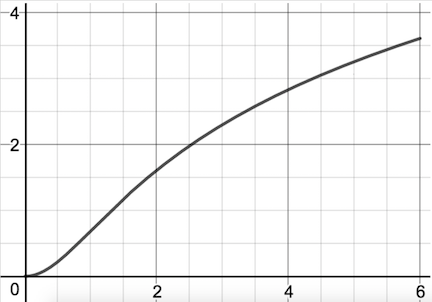
\includegraphics [scale=0.5]{Area-Ex3.pdf} %%This is on my computer, not sure if it's in GitHub%%

\begin{multipleChoice}
	\choice {$6$}
	\choice [correct]{$12$}
	\choice {$18$}
	\choice {$24$}
\end{multipleChoice}
\end{problem}


%%Problem 4%%
\begin{problem}
Consider $Q(x)=\displaystyle\frac{1}{x^2+1}$

\begin{question}
What is the domain of $Q$?
\begin{multipleChoice}
	\choice {$(-\infty,-1)\cup(-1,1)\cup(1,\infty)$}
	\choice {$(-\infty,0)\cup(1,\infty)$}
	\choice [correct]{$(-\infty,\infty)$}
	\choice {$(-\infty,-1)\cup(-1,\infty)$}
\end{multipleChoice}
\end{question}

\begin{question}
What are the critical points of $Q$?
\begin{multipleChoice}
	\choice {$x=-1$, $x=1$}
	\choice [correct]{$x=0$}
	\choice {$x=-1$, $x=1$, $x=0$}
	\choice {$Q(x)$ does not have any critical points.}
\end{multipleChoice}
\end{question}

\end{problem}


%%Problem 5%%
\begin{problem}
The function $\displaystyle g(x) = \frac{1}{24}x^3+\sqrt{x}$ is concave down for all $x$ in the interval
\begin{multipleChoice}
	\choice [correct]{$(0,1)$}
	\choice {$(1,\infty)$}
	\choice {$(0,\infty)$}
	\choice {$g(x)$ is never concave down.}
\end{problem}


%%Problem 6%%
\begin{problem}
What are the inflection points of $F(x)=x^4-4x^3+6x^2+1$?
\begin{multipleChoice}
	\choice {$x=0$}
	\choice {$x=1$}
	\choice [correct]{$F(x)$ does not have any inflection points.}
\end{multipleChoice}
\end{problem}


%%Problem 7%%
\begin{problem}
Suppose that $f'(x)$ is continuous and differentiable on its domain, $f'(B)=0$, and $f(x)$ has a local minimum at $x=B$. Then which of the following statements is true? 
\begin{selectAll}
	\choice [correct]{$f'(x)$ changes from negative to positive at $x=B$ (as $x$ increases).}
	\choice {$f'(x)$ changes from positive to negative at $x=B$ (as $x$ increases).}
	\choice {$f''(B)<0$.} 
	\choice [correct]{$f''(B)>0$.}
	\choice {$f''(B)=0$.}
	\choice {None of the above.}
\end{selectAll}
\end{problem}














\end{document}